\subsection{题目描述}
\noindent
The interior of a $d$-dimensional hypersphere of unit radius is defined by the condition
$x_1^2 + x_2^2 + \cdots + x_d^2 \leq 1$. Write a program that finds the volume of a hypersphere
using a Monte Carlo method. Test your program for $d=2$ and $d=3$ and then calculate the volume
for $d=4$ and $d=5$, compare your results with the exact results.


\subsection{程序描述}
本程序用于估计$n$维单位超球体的体积,并通过蒙特卡洛方法进行比较分析。主要功能包括:
\begin{itemize}
    \item 动画演示2维和3维下的蒙特卡洛采样过程。
    \item 使用简单的均匀采样和重要性采样两种方法对1到20维的单位超球进行体积估计,并与理论值比较。
    \item 在高维数据下通过PCA降维进行可视化,并绘制误差、计算时间等分析图表。
\end{itemize}
在这里,$n$维单位超球体指的是半径为1的$n$维球体(n-ball),即集合
\(
\{x \in \mathbb{R}^n : \|x\| \le 1\}
\)
其理论体积公式为:
\[
    V_n = \frac{\pi^{n/2}}{\Gamma\left(\frac{n}{2} + 1\right)}
\]
\subsubsection{简单均匀采样}
在$\mathbb{R}^n$空间中从$[-1, 1]^n$的均匀分布中采样\texttt{num\_samples}个点,统计其中有多少点在单位超球体内,计算落入比例与超立方体的体积$2^n$,从而估计体积。该方法在高位空间收敛较慢,误差较大,因为高维空间中单位超球体的体积占整个超立方体的比例很小,采样集中在浅表面。
\subsubsection{重要性采样}
本程序的重要性采样使用多元正态分布$N(0, \sigma^2 I)$作为提议分布$q(x)$进行采样,即
\[
    q(x) = \frac{1}{(2\pi \sigma^2)^{n/2}} \exp\left(-\frac{\|x\|^2}{2\sigma^2}\right)
\]
采样后统计各点到原点的距离,定义指示函数$ f(x) = 1_{B_n}(x) $表示该点是否在单位球内(在则为1,否则0)。该提议分布采样的点集中在原点附近,更容易采样到单位球内的点,从而提高采样效率。若定义相对于$Lebesgue$测度$dx$的目标分布$p(x) \equiv 1$(其不满足归一化,故不是狭义的概率分布),则可将体积估计问题转化为期望值问题:
\[
    \int f(x)p(x)dx = \int f(x)\cdot 1 \, dx = \int_{\mathbb{R}^n} f(x)dx = V_n
\]
重要性采样通常要求良好概率分布的提议分布$q(x)$,满足\(\int q(x)dx=1\),将难以直接采样的期望问题进行转化
\[
    \mathbb{E}_p[f(X)] = \int f(x) \frac{p(x)}{q(x)} q(x) dx = \mathbb{E}_q\left[f(X)\frac{p(X)}{q(X)}\right]
\]
本题的目标分布为常函数1,故只需要如下估计超球体积
\[
    \hat{V_n} = \frac{1}{N}\sum_{i=1}^N \frac{f(x_i)}{q(x_i)}
\]
本程序还有一些辅助的可视化工具,在此不一一赘述。用户在\texttt{src}目录下运行\ccmd{python -u hypersphere.py}即可运行程序,需安装辅助计算的\texttt{numpy}库与绘图用的\texttt{matplotlib}库,对于重要性采样,因追求较高精度,默认采样点数较多,故运行时间较长,故建议安装\texttt{tqdm}库以显示进度条。在主菜单中,用户可以选择
\begin{itemize}
    \item[(1)] 动画演示(仅2维或3维)
    \item[(2)] 简单均匀采样分析(1~20维),并可选择可视化采样点。
    \item[(3)] 重要性采样分析(1~20维),并可选择可视化采样点。
\end{itemize}
在二级菜单中还将可以自定义一些参数,如采样点数、最大计算维度,提议分布标准差与试验次数等,详见下文的伪代码与结果示例。
\subsection{伪代码}
Powered by \href{https://chatgpt.com/g/g-xJJAA2awf-latex-pseudocode-generator}{\LaTeX \ pseudocode generator}

\begin{algorithm}[H]
    \SetAlgoLined
    \KwIn{$max\_dim$, $num\_samples$, $num\_trials$, $method$, $\sigma$ (optional)}
    \KwOut{Results for dimensions $1$ to $max\_dim$}

    \For{$d \gets 1$ \KwTo $max\_dim$}{
        $exact \gets exact\_volume(d)$; $estimates \gets []$\;
        \For{$trial \gets 1$ \KwTo $num\_trials$}{
            \If{$method = \text{uniform}$}{
                $v \gets monte\_carlo\_uniform(d, num\_samples)$\;
            }
            \Else{
                $v \gets importance\_sampling\_volume(d, num\_samples, \sigma)$\;
            }
            $estimates.append(v)$\;
        }
        $mean, std, rel\_err \gets analyze(estimates, exact)$ \tcp*[r]{Compute statistics}
    }
    \Return{All results}\;
    \caption{Main Program}
\end{algorithm}

\begin{algorithm}[H]
    \SetAlgoLined
    \KwIn{$n$, $num\_samples$}
    \KwOut{Estimated volume}

    $points \gets \text{random uniform in } [-1, 1]^n$\;
    $distances \gets ||points||^2$\;
    $count \gets \text{sum}(distances \leq 1)$\;
    \Return{$2^n \cdot (count / num\_samples)$}\;
    \caption{Uniform Sampling}
\end{algorithm}

\begin{algorithm}[H]
    \SetAlgoLined
    \KwIn{$n$, $num\_samples$, $\sigma$}
    \KwOut{Estimated volume}

    $samples \gets \text{normal}(mean=0, cov=\sigma^2I_n, num\_samples)$\;
    $distances \gets ||samples||^2$\;
    $f_x \gets (distances \leq 1)$; $q_x \gets (2\pi\sigma^2)^{-n/2} \cdot e^{-distances / (2\sigma^2)}$\;
    $weights \gets f_x / q_x$\;
    \Return{$\text{mean}(weights)$}\;
    \caption{Importance Sampling}
\end{algorithm}
\subsection{结果示例}
\subsubsection{简单均匀采样}
\begin{figure}[H]
    \centering
    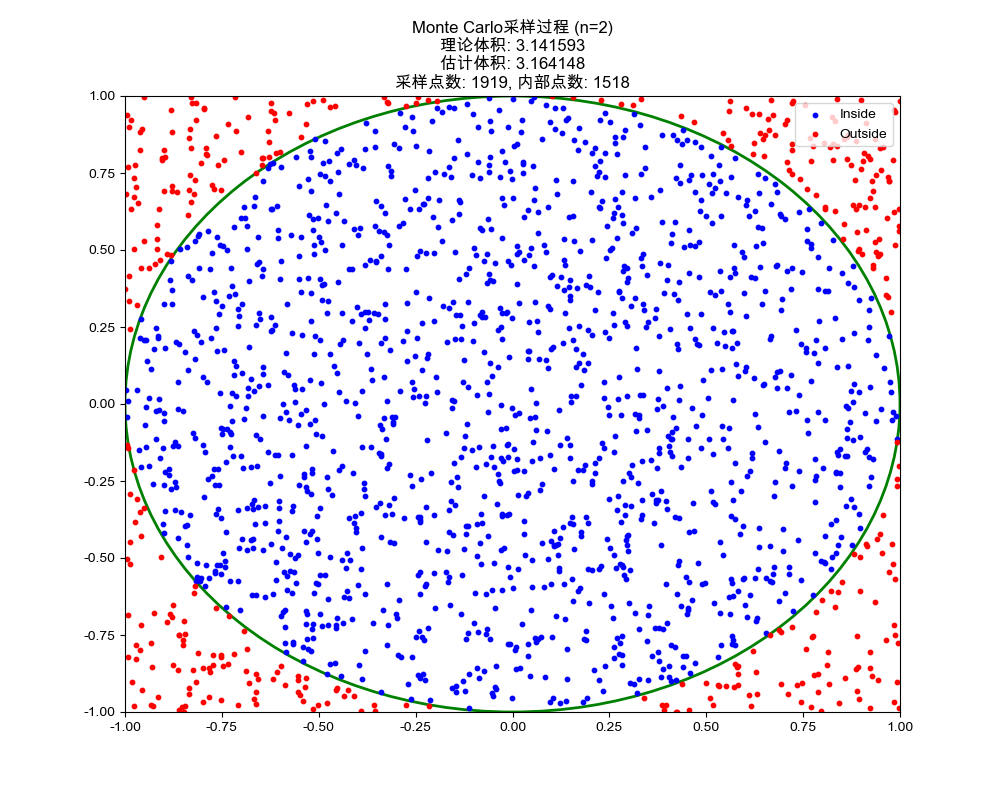
\includegraphics[width=0.45\textwidth]{Problem_1/figs/2d_anim.png}
    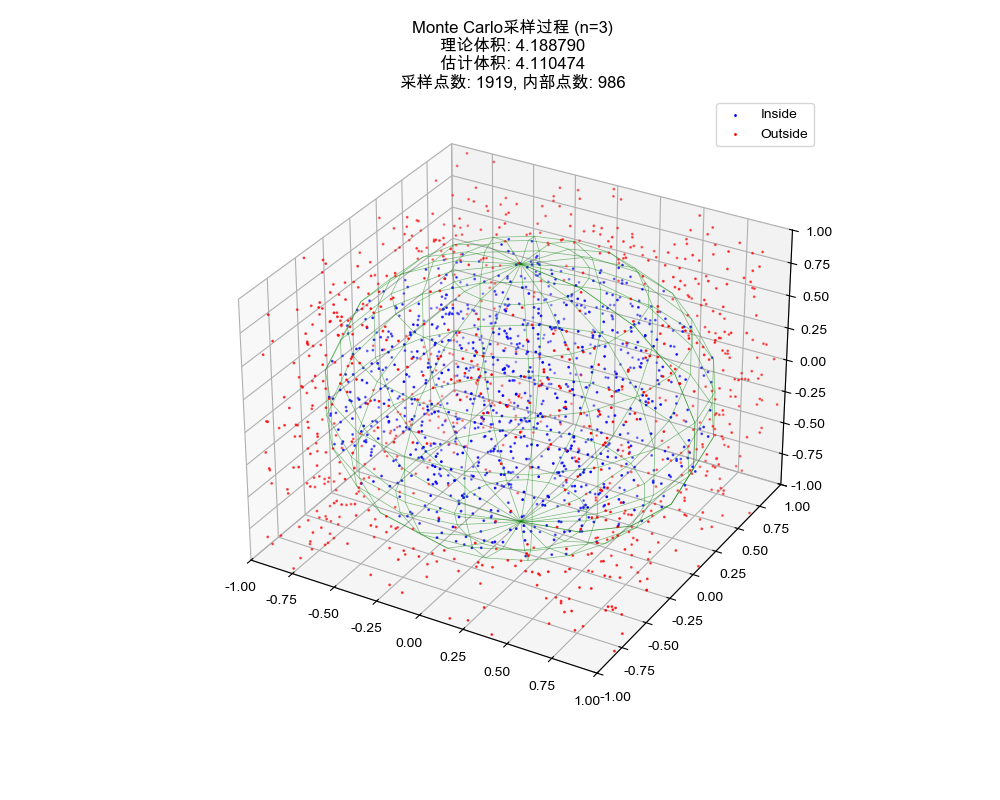
\includegraphics[width=0.45\textwidth]{Problem_1/figs/3d_anim.png}
    \caption{二维与三维简单采样动画截图}
\end{figure}
\begin{figure}[H]
    \centering
    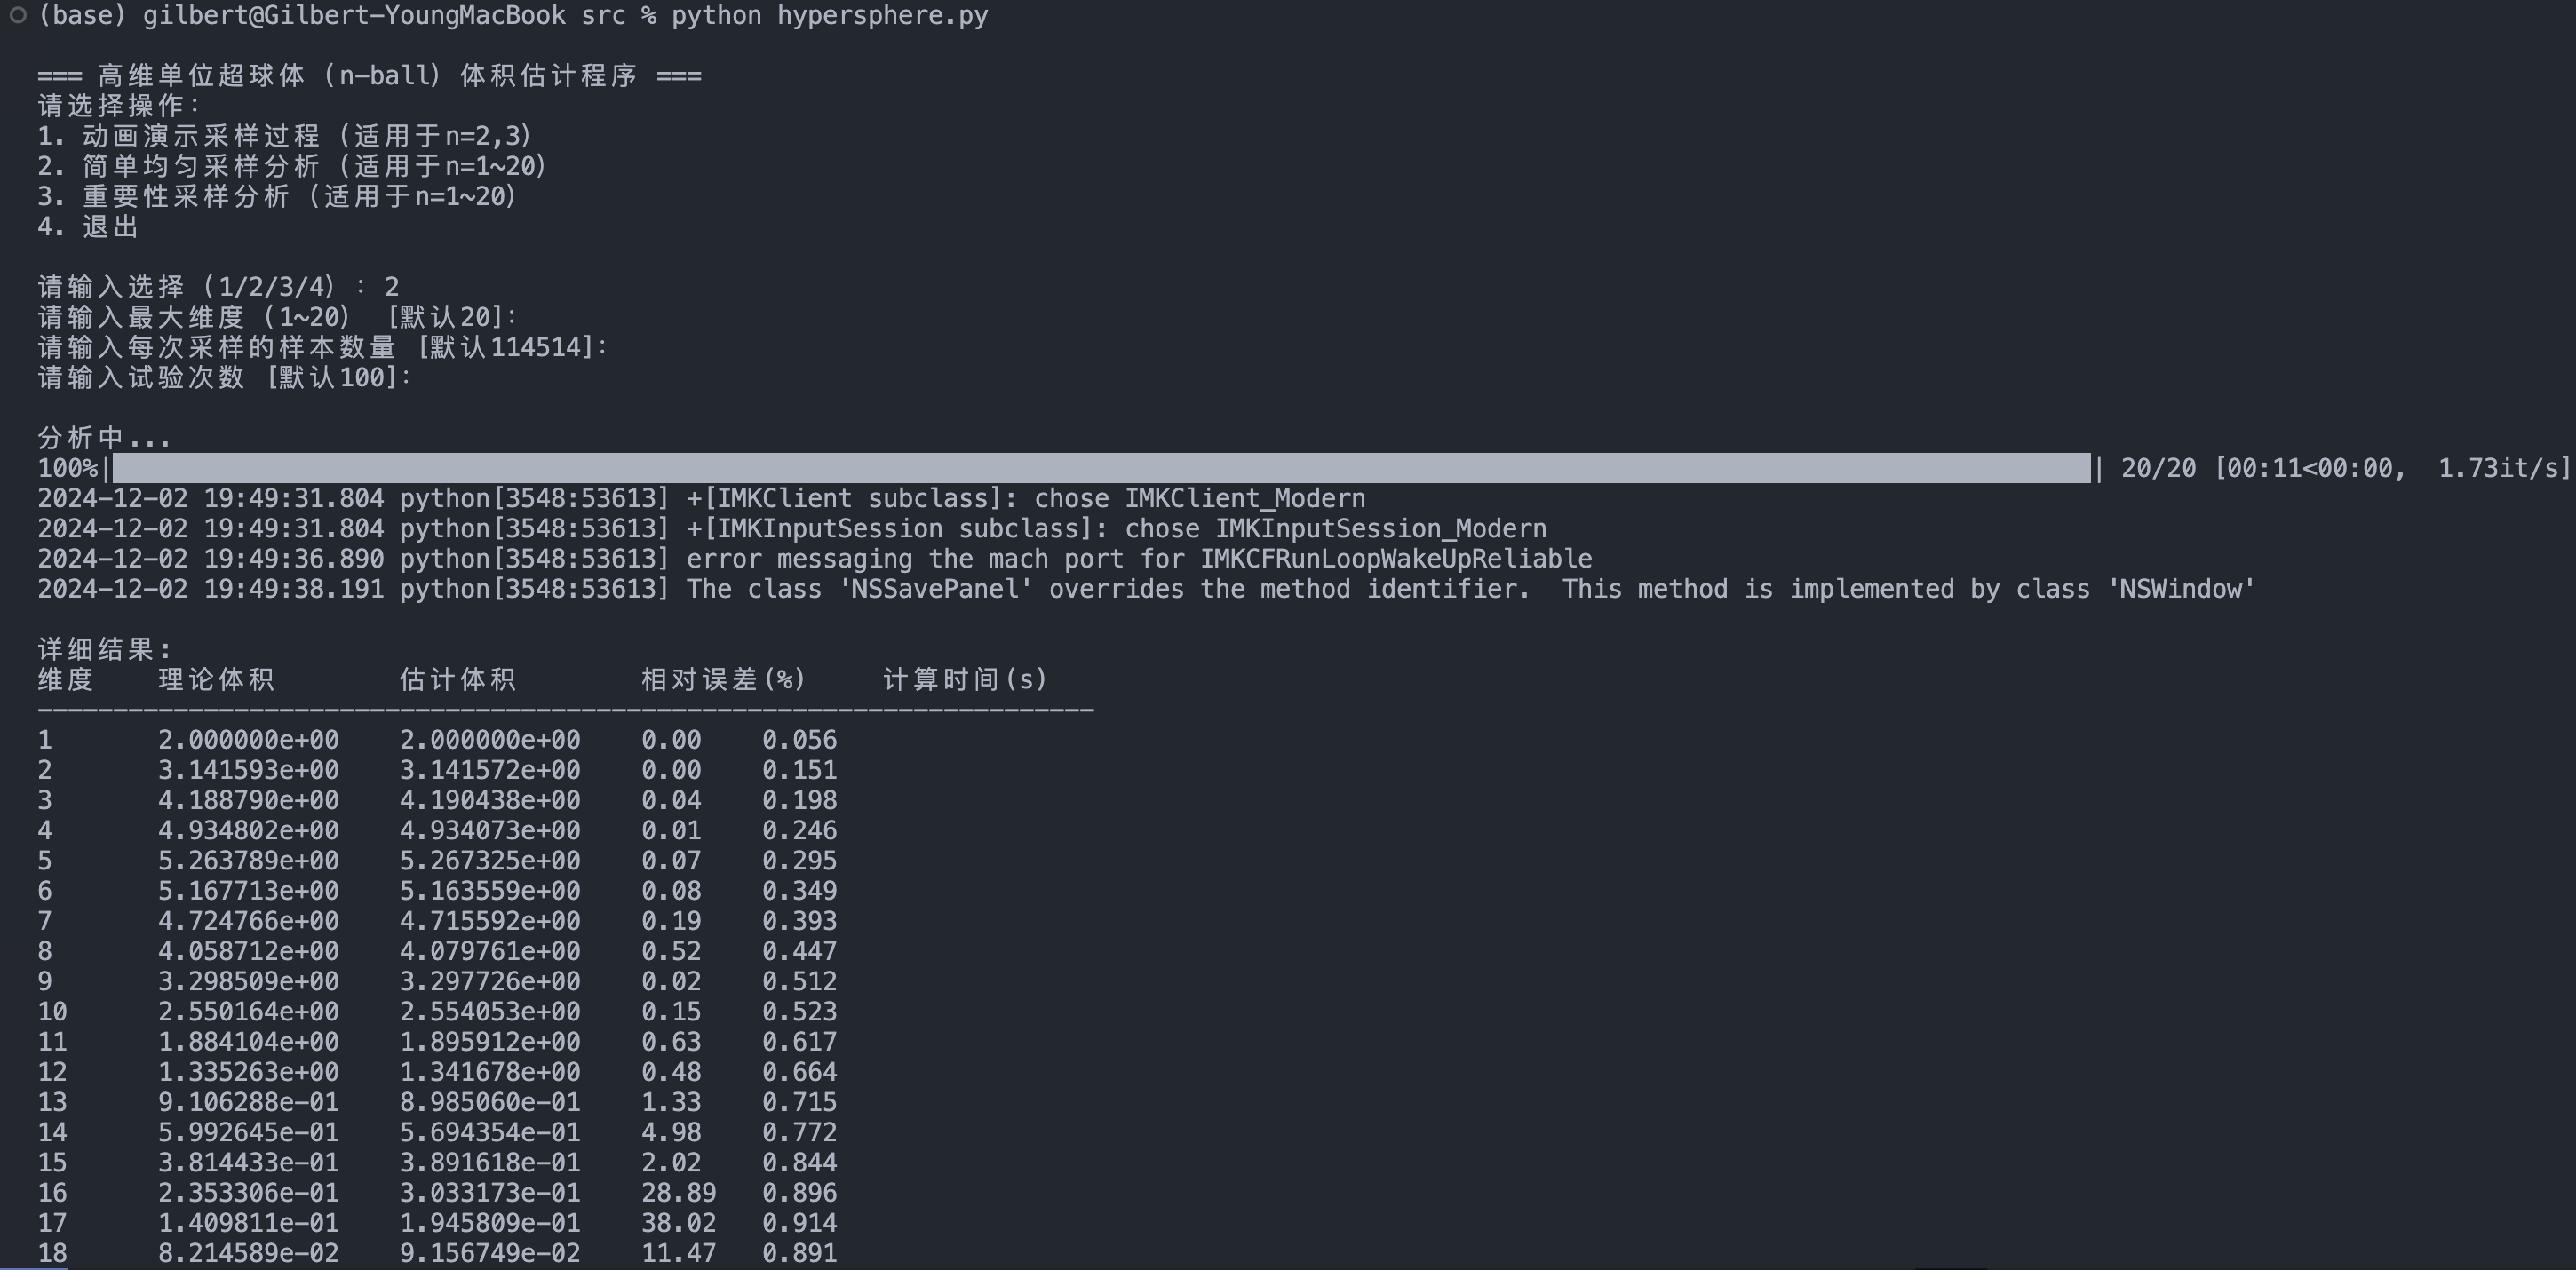
\includegraphics[width=1.0\textwidth]{Problem_1/figs/simple_terminal.png}
    \caption{简单均匀采样终端输出}
\end{figure}

\begin{figure}[H]
    \centering
    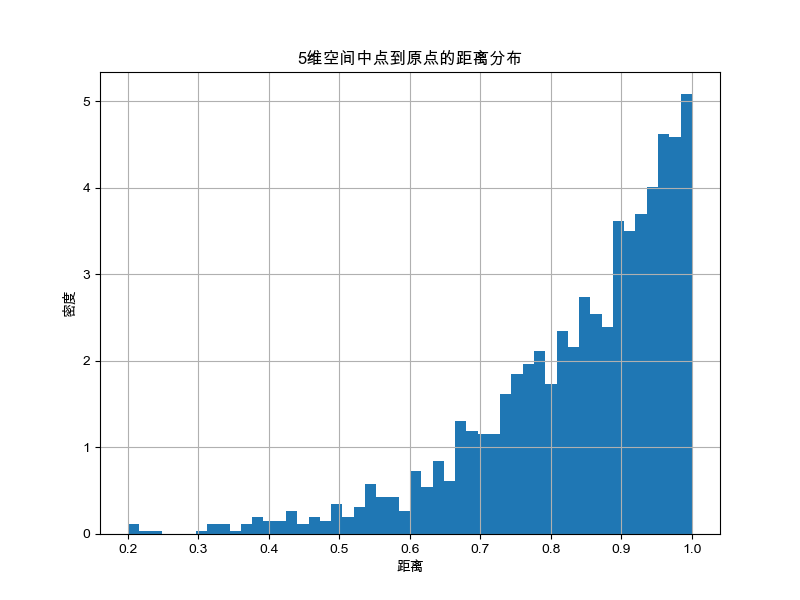
\includegraphics[width=0.48\textwidth]{Problem_1/figs/simple_5d_dis.png}
    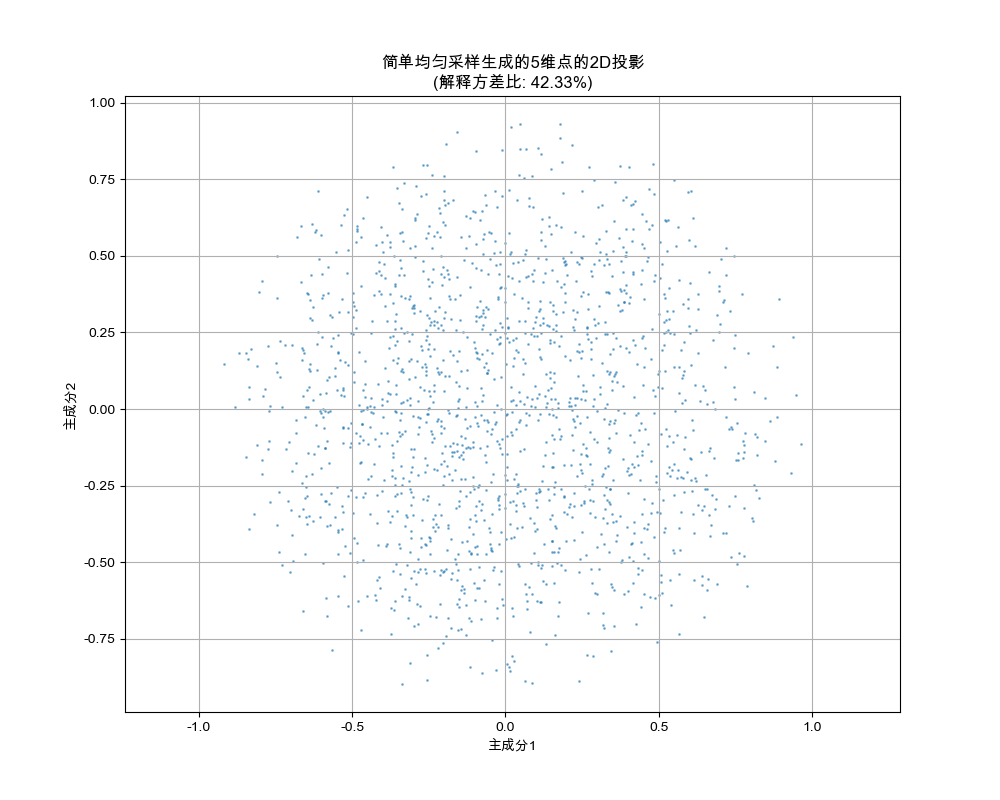
\includegraphics[width=0.48\textwidth]{Problem_1/figs/simple_5d_pca.png}
    \caption{简单均匀采样点分布与PCA主成分分析(5维)}
\end{figure}

\begin{figure}[H]
    \centering
    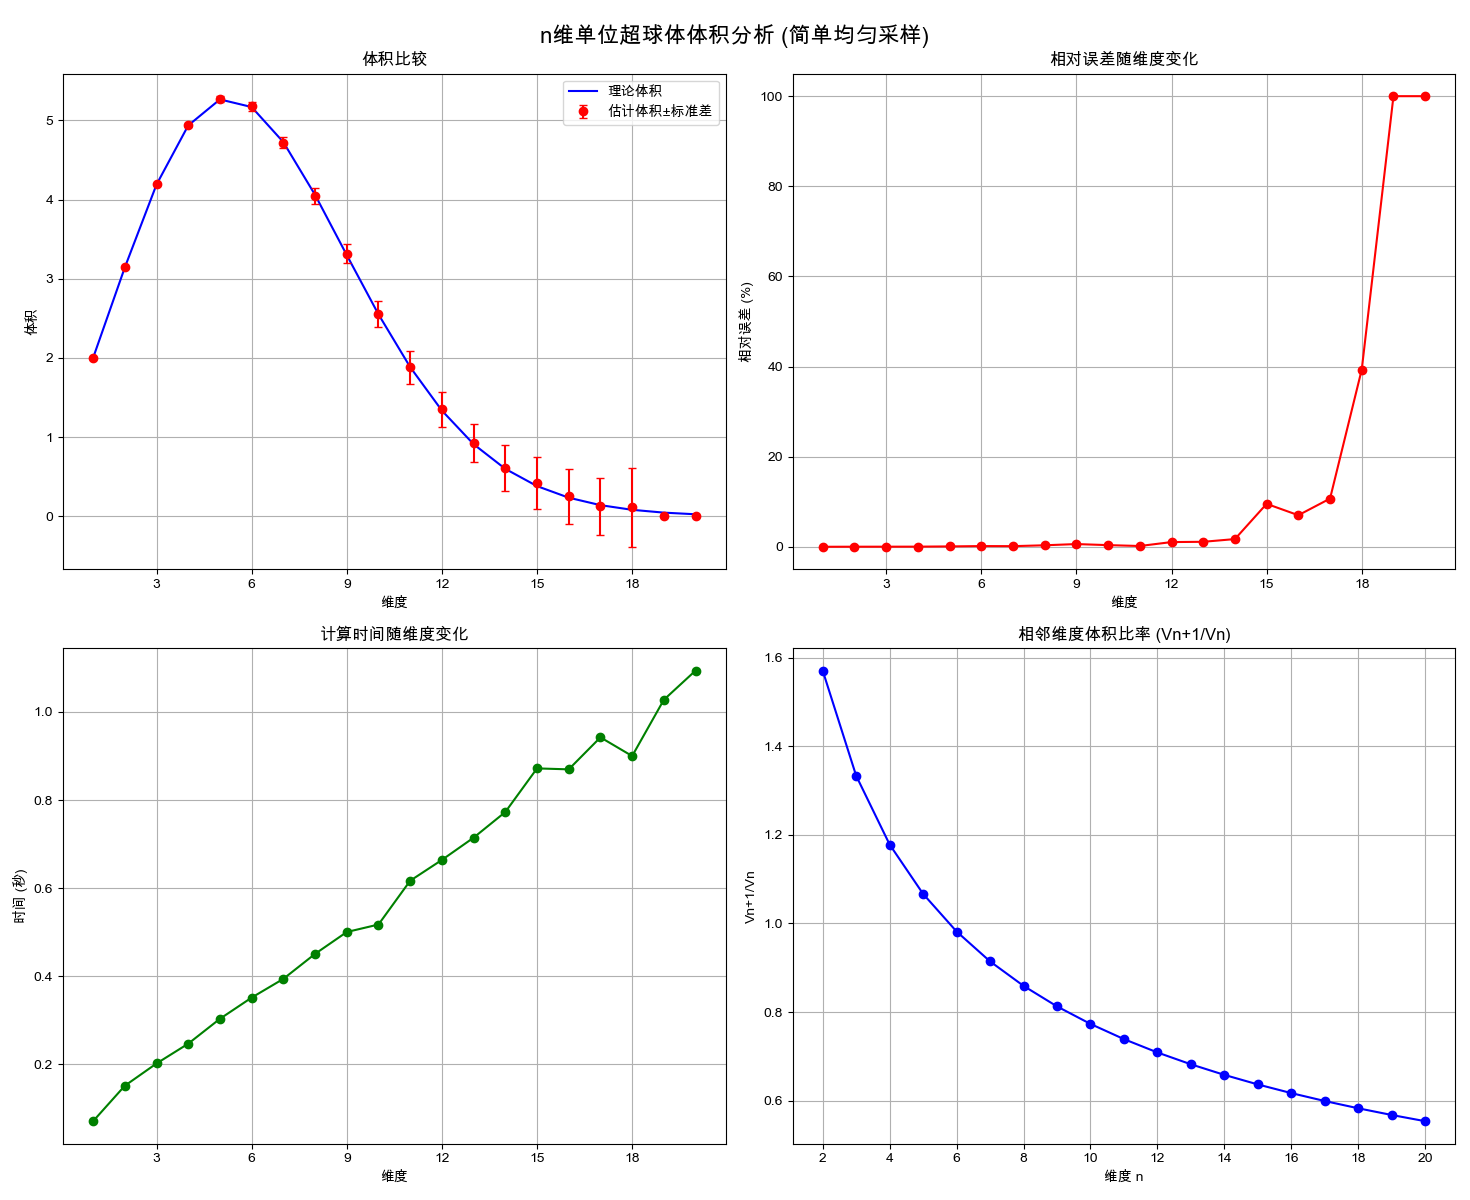
\includegraphics[width=1.0\textwidth]{Problem_1/figs/simple.png}
    \caption{简单均匀采样结果分析}
\end{figure}
可见在高维还是表现不容乐观的,需要借助重要性采样。

\subsubsection{重要性采样}
\begin{figure}[H]
    \centering
    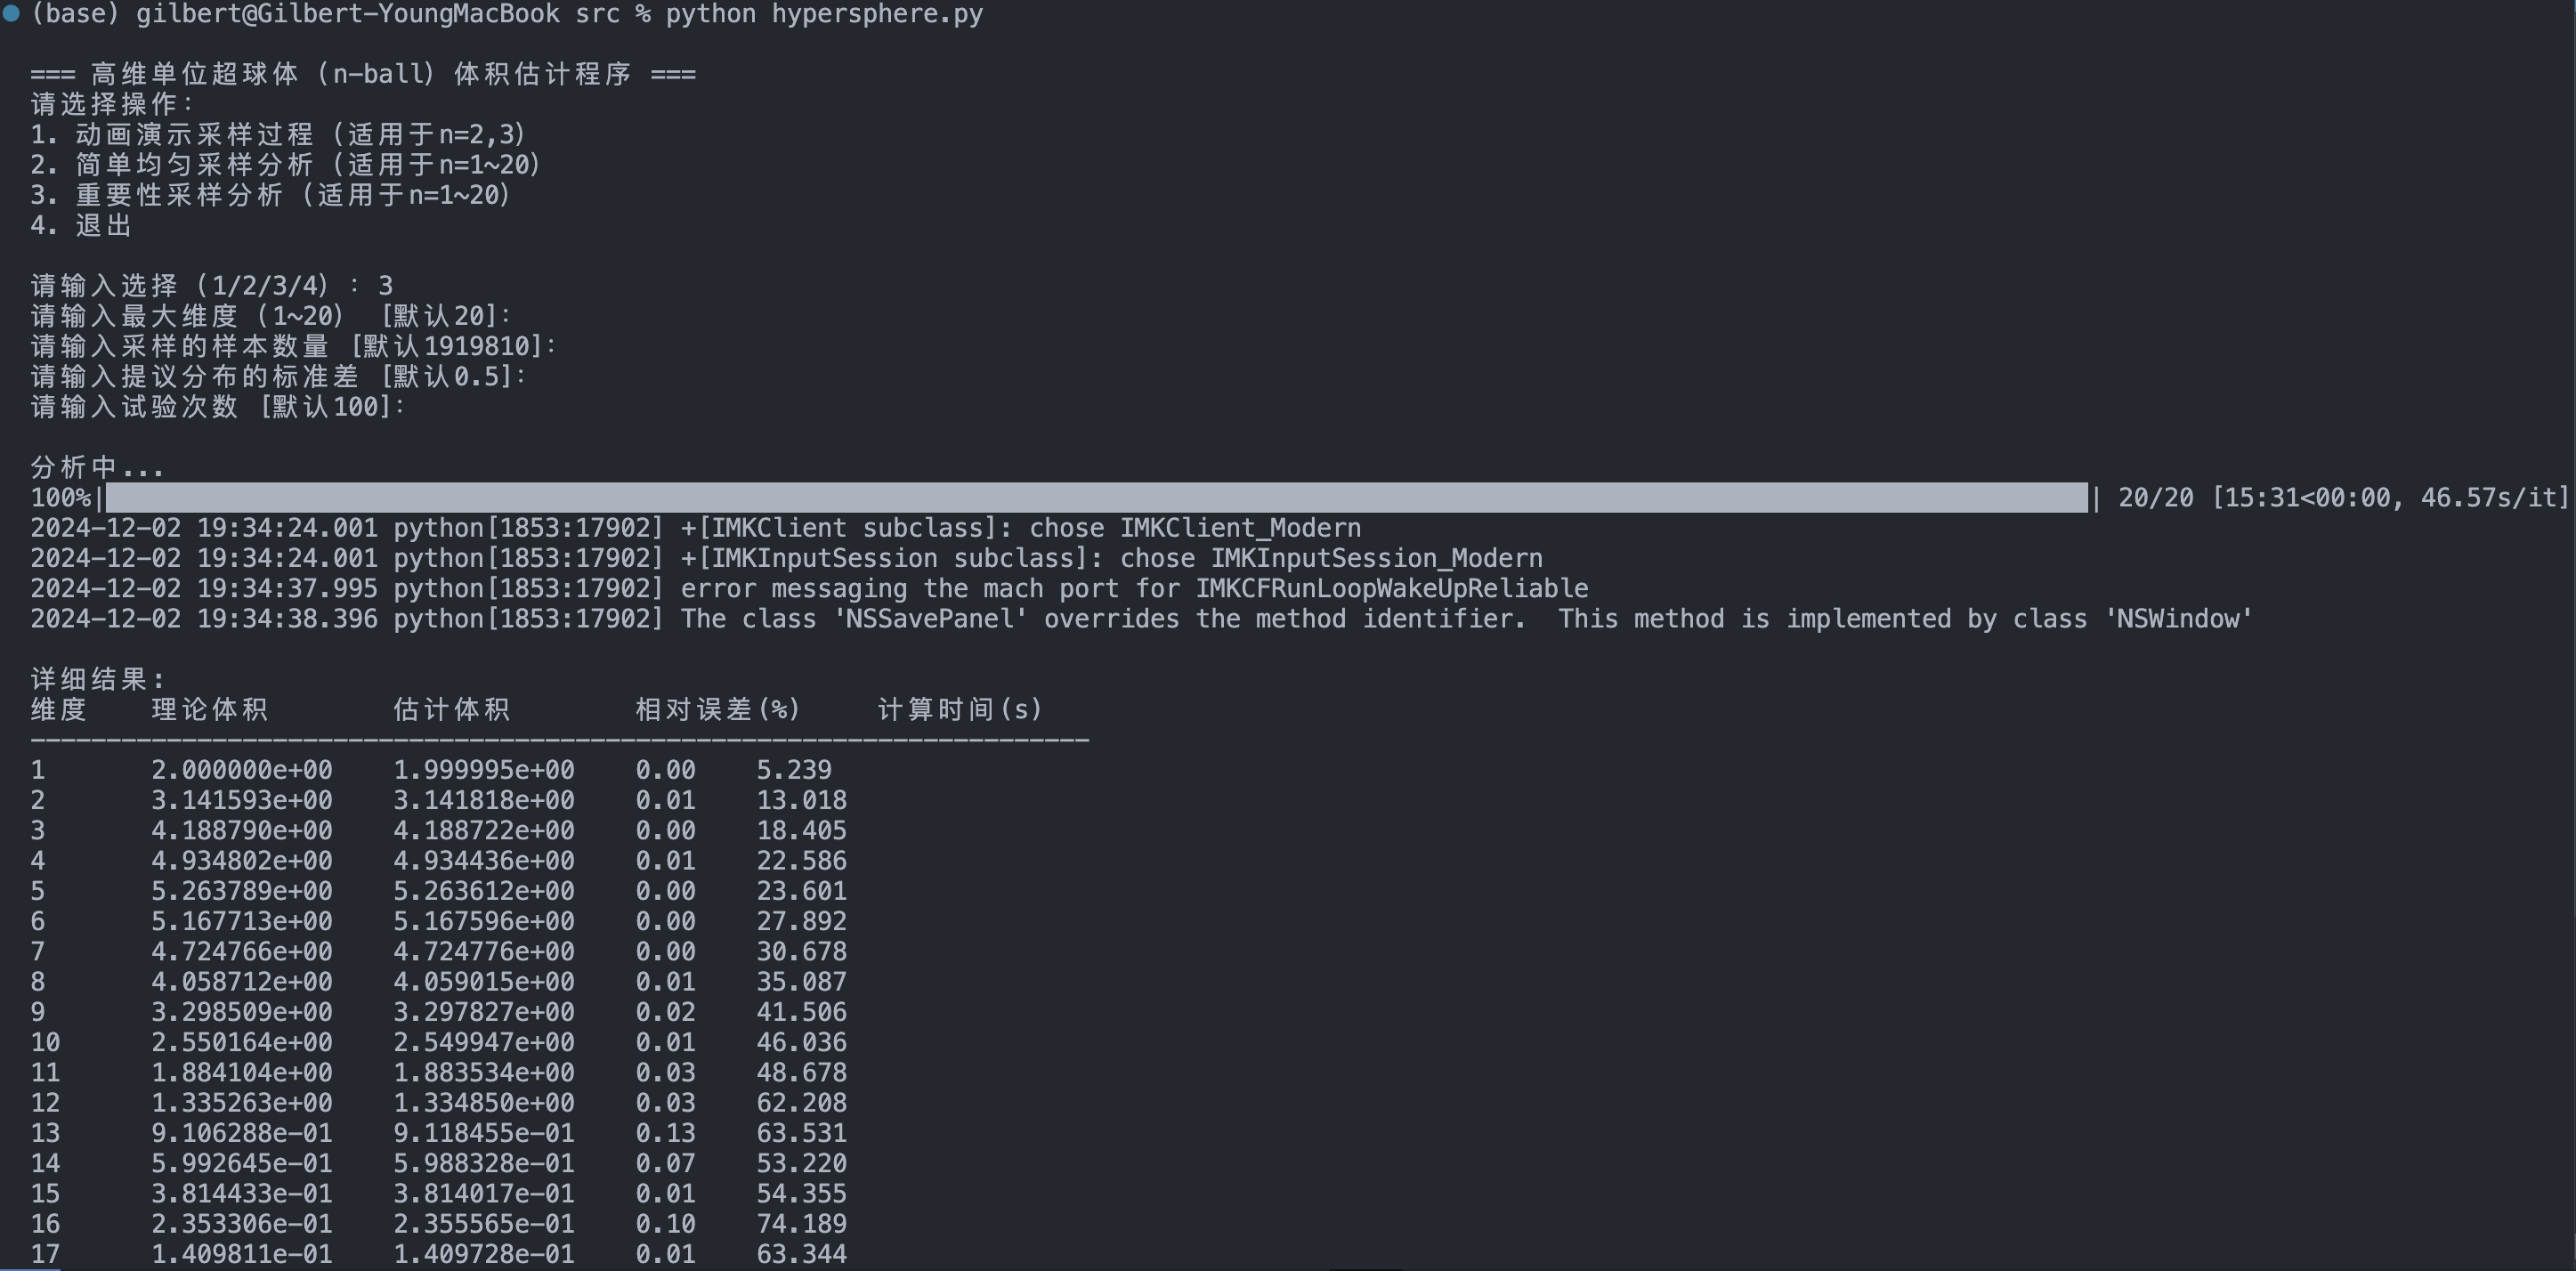
\includegraphics[width=1.0\textwidth]{Problem_1/figs/important_terminal.png}
    \caption{重要性采样终端输出}
\end{figure}

\begin{figure}[H]
    \centering
    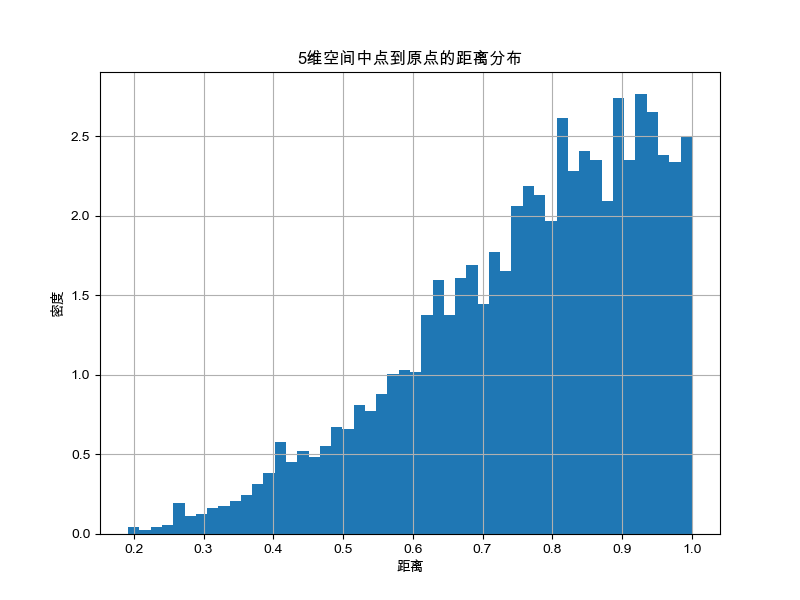
\includegraphics[width=0.48\textwidth]{Problem_1/figs/important_5d_dis.png}
    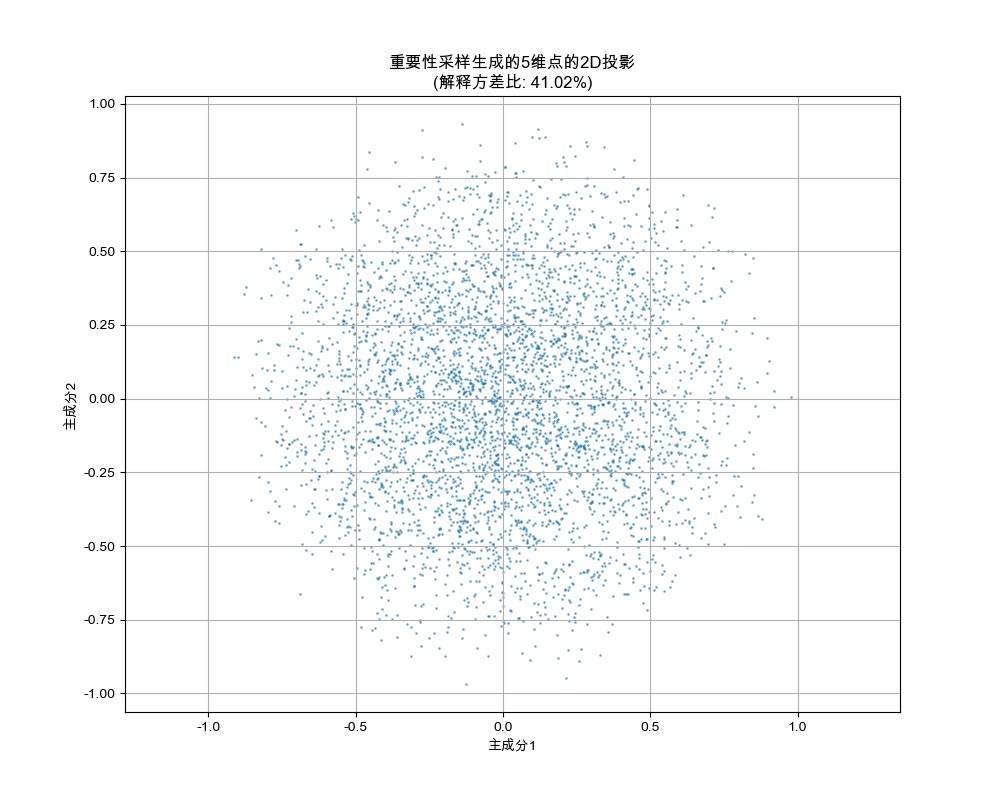
\includegraphics[width=0.48\textwidth]{Problem_1/figs/important_5d_pca.png}
    \caption{重要性采样点分布与PCA主成分分析(5维)}
\end{figure}
可见采样点明显向原点附近区域迁移。

\begin{figure}[H]
    \centering
    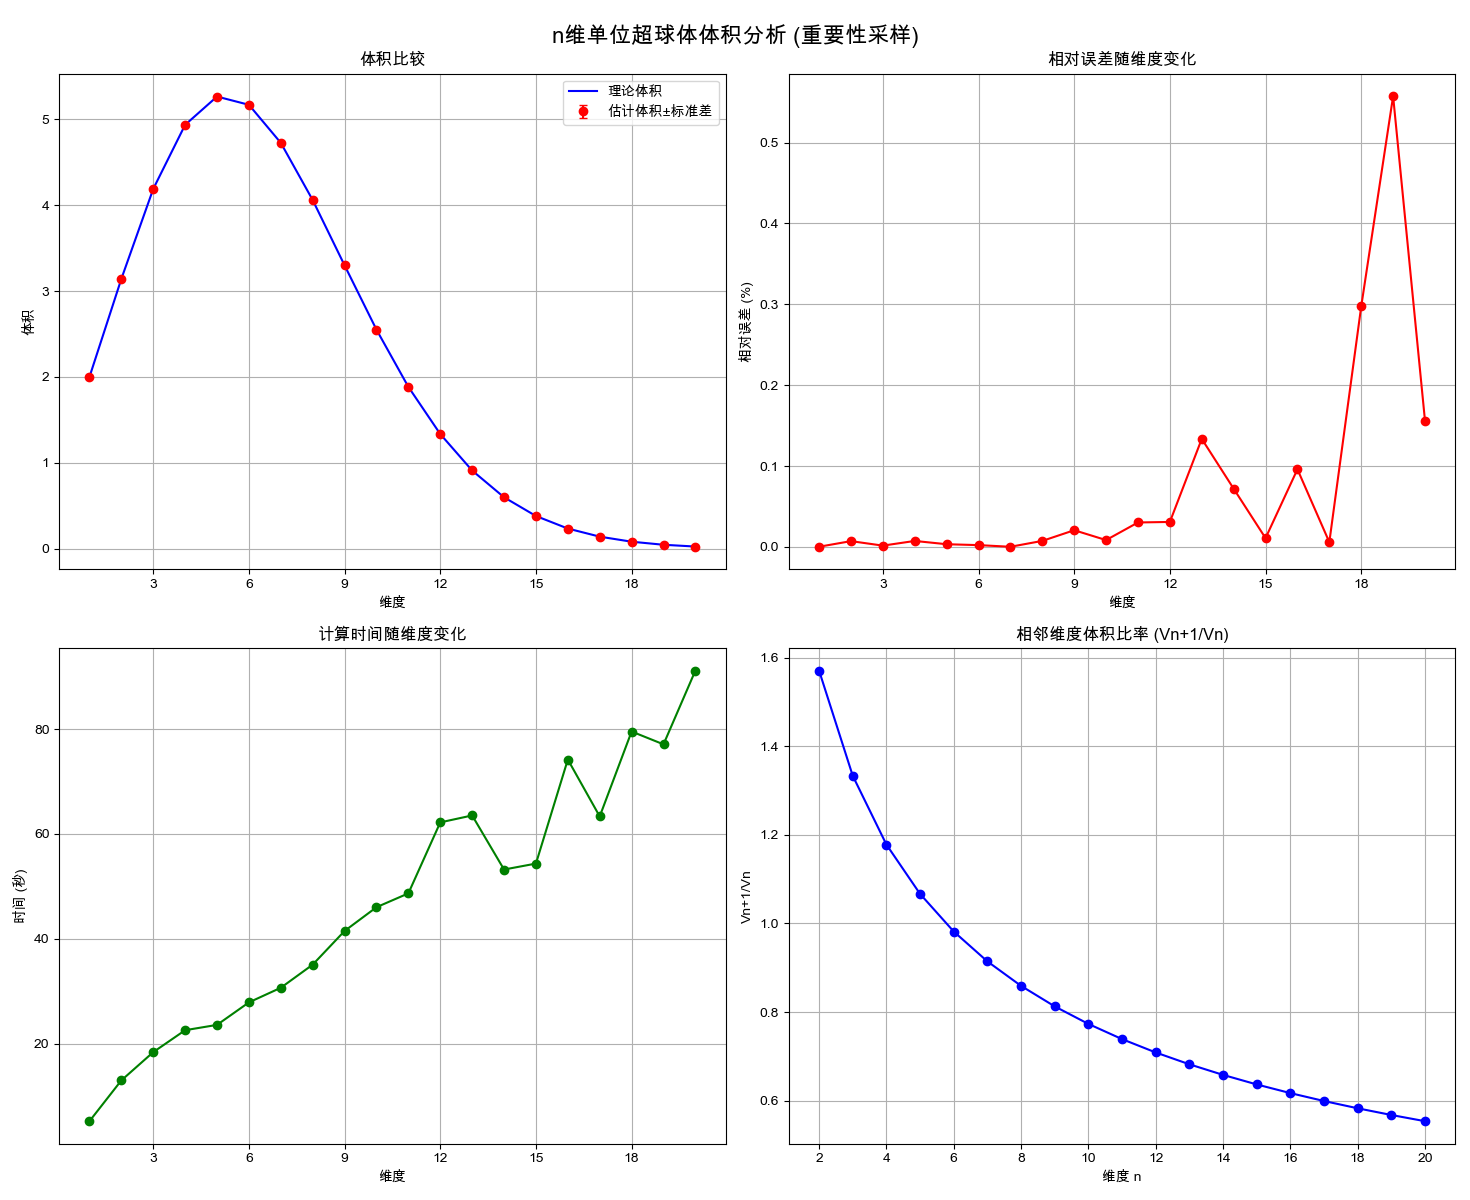
\includegraphics[width=1.0\textwidth]{Problem_1/figs/important.png}
    \caption{重要性采样结果分析}
\end{figure}
相对误差以解析解为标准,最大值仅为千分之十三,相对于简单均匀采样有了质的提升。计算时间大幅增加是因为不小心将采样点数从$114514$提升至$1919810$,增加了一个数量级以上。对于不同维度,还可以精细调整提议分布标准差以获得更好的效果。